\documentclass[11pt,varwidth=\maxdimen]{standalone}
%\documentclass{article}
\usepackage[english]{babel}	
\usepackage[utf8]{inputenc}	% Allows for writing special charachters in the tex-file 

\usepackage{amsfonts,amsmath,amssymb,bm,mathrsfs,mathtools,dsfont} 	% Standard mathematics 


% Fonts
% \DeclareMathAlphabet{\mathsfit}{OT1}{lmss}{m}{sl}
% \DeclareMathAlphabet{\mathsfbf}{OT1}{lmss}{bx}{n}
% \DeclareMathAlphabet{\mathsfbfit}{OT1}{lmss}{bx}{sl}
 
% \DeclareMathVersion{sectionmath}
% \SetSymbolFont{operators}{sectionmath}{OT1}{cmbr}{m}{n}
% \SetSymbolFont{letters}{sectionmath}{OML}{cmbrm}{b}{it}
% \SetSymbolFont{symbols}{sectionmath}{OMS}{cmbrs}{m}{n}
% \DeclareMathVersion{normalmath}
% \SetSymbolFont{operators}{normalmath}{OT1}{cmbr}{m}{n}
% \SetSymbolFont{letters}{normalmath}{OML}{cmbrm}{m}{it}
% \SetSymbolFont{symbols}{normalmath}{OMS}{cmbrs}{m}{n}

% \mathversion{normalmath}
% \renewcommand{\familydefault}{\sfdefault} %Use sans serif 


\usepackage{xcolor}
\definecolor{rmp}{RGB}{41, 43, 133}
\definecolor{myblue}{rgb}{0.24, 0.36, 0.44}
\definecolor{mygreen}{rgb}{0.367, 0.473, 0.0}
\definecolor{darkcoral}{rgb}{0.8, 0.36, 0.27}
\definecolor{darktangerine}{rgb}{1.0, 0.66, 0.07}
\definecolor{amber}{rgb}{1.0, 0.75, 0.0}


\usepackage{tikz}
\usetikzlibrary{positioning,shapes,calc,arrows.meta,decorations.pathreplacing,calligraphy}

\newcommand{\coord}[4]{({(#1)+(#3)*cos(#4)},{(#2)+(#3)*sin(#4)})}


\newcommand{\sscript}[1]{{\scriptscriptstyle \mathrm{#1}}}
\newcommand{\EFT}{\sscript{EFT}}


% % % % % % Commands % % % % % % %

\begin{document}
	% Normal page width =15.4
	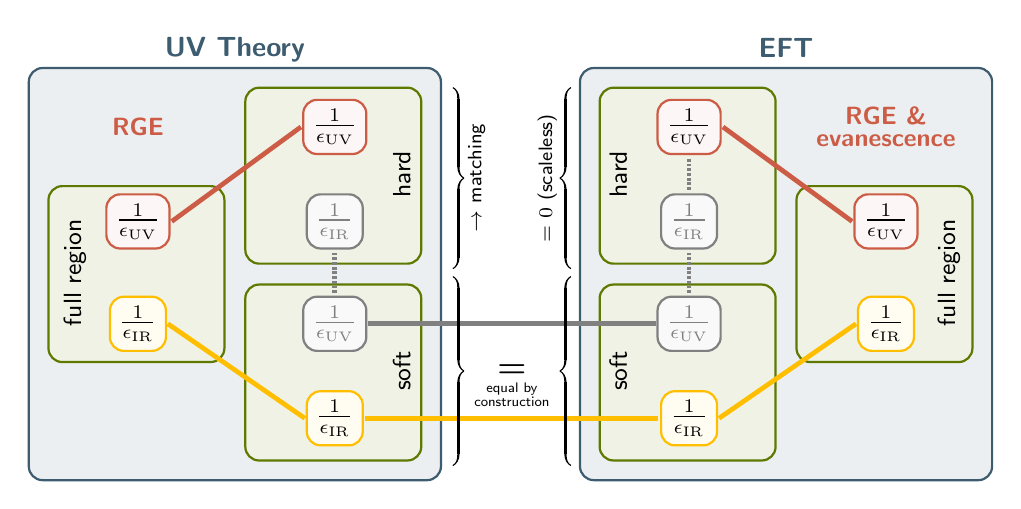
\begin{tikzpicture} [
			scale = 1,
			>={Stealth[]},
			frame/.style={draw, 
					rectangle, 
					text centered, 
					minimum size=1ex, 
					rounded corners= 5pt,
					draw= myblue,
					fill= myblue!10!white,
                    font=\sffamily,
                    anchor=south west},
            frame2/.style={draw, 
					rectangle, 
                    text centered,
					minimum size=1ex, 
					rounded corners= 5pt,
					draw= mygreen,
					fill= mygreen!10!white,
                    font=\sffamily,
                    anchor=south west},
            frame3/.style={draw, 
					rectangle, 
                    text centered,
					minimum size=1ex, 
					rounded corners= 5pt,
					draw= gray,
					fill= gray!5!white,
                    font=\sffamily,
                    text= gray,
                    anchor=center},
            frameUV/.style={draw, 
					rectangle, 
                    text centered,
					minimum size=1ex, 
					rounded corners= 5pt,
					draw= darkcoral,
					fill= darkcoral!5!white,
                    font=\sffamily,
                    anchor=center},
            frameIR/.style={draw, 
					rectangle, 
                    text centered,
					minimum size=1ex, 
					rounded corners= 5pt,
					draw= amber,
					fill= amber!5!white,
                    font=\sffamily,
                    anchor=center},
            mytext/.style={ 
					text centered, 
                    font=\bf\sffamily,
                    text= myblue,
                    anchor=south west},
            text2/.style={ 
					text centered, 
                    font=\small\sffamily},
			output/.style={frame, 
%					draw= darkred, 
%					fill= darkred!20!white,
				},
			to/.style={->, line width= 1.5pt}
		] \pgfsetlinewidth{.8pt} %Set default linewidth to be thick

        
        % BSM block
        \node[frame, text width= 5cm, text height= 5cm] at (0,0) { };
        \node[font=\bf\sffamily, text= myblue, text centered, text width= 5cm, anchor=south west] at (0,5.2) {UV Theory};

        \node[frame2, text width= 2cm, text height= 2cm] at (0.25,1.5) {};
        \node[frameUV] at (1.4,3.3) {$\frac{1}{\epsilon_{\mathrm{UV}}}$};
        \node[frameIR] at (1.4,2.0) {$\frac{1}{\epsilon_{\mathrm{IR}}}$};
        \node[text2, rotate=90] at (0.6,2.65) {full region};
        
        \node[frame2, text width= 2cm, text height= 2cm] at (2.75,2.75) {};
        \node[frameUV] at (3.9,4.5) {$\frac{1}{\epsilon_{\mathrm{UV}}}$};
        \node[frame3] at (3.9,3.3) {$\frac{1}{\epsilon_{\mathrm{IR}}}$};
        \node[text2, rotate=90] at (4.75,3.9) {hard};
        
        \node[frame2, text width= 2cm, text height= 2cm] at (2.75,0.25) {};
        \node[frame3] at (3.9,2) {$\frac{1}{\epsilon_{\mathrm{UV}}}$};
        \node[frameIR] at (3.9,0.8) {$\frac{1}{\epsilon_{\mathrm{IR}}}$};
        \node[text2, rotate=90] at (4.75,1.4) {soft};

        % \draw[->] (1.8,3.35) -- (3.5,4.5) ;
        \node[text2, text= darkcoral, font=\bf\small\sffamily, align=center] at (1.4,4.5) {RGE} ;
        \draw[darkcoral, line width=0.6mm] (1.83,3.3) -- (3.47,4.5) ;
        \draw[amber, line width=0.6mm] (1.78,2.0) -- (3.52,0.8) ;
        \draw[gray,line width=0.6mm, dash pattern={on 1pt off 0.7pt}] (3.9,2.39) -- (3.9,2.92) ;


        % SMEFT block
        \node[frame, text width= 5cm, text height= 5cm] at (7,0) { };
        \node[font=\bf\sffamily, text= myblue, text centered, text width= 5cm, anchor=south west] at (7,5.25) {EFT};
        
        \node[frame2, text width= 2cm, text height= 2cm] at (9.75,1.5) {};
        \node[frameUV] at (10.9,3.3) {$\frac{1}{\epsilon_{\mathrm{UV}}}$};
        \node[frameIR] at (10.9,2.0) {$\frac{1}{\epsilon_{\mathrm{IR}}}$};
        \node[text2, rotate=90] at (11.7,2.65) {full region};

        \node[frame2, text width= 2cm, text height= 2cm] at (7.25,2.75) {};
        \node[frameUV] at (8.4,4.5) {$\frac{1}{\epsilon_{\mathrm{UV}}}$};
        \node[frame3] at (8.4,3.3) {$\frac{1}{\epsilon_{\mathrm{IR}}}$};
        \node[text2, rotate=90] at (7.5,3.9) {hard};

        \node[frame2, text width= 2cm, text height= 2cm] at (7.25,0.25) {};
        \node[frame3] at (8.4,2) {$\frac{1}{\epsilon_{\mathrm{UV}}}$};
        \node[frameIR] at (8.4,0.8) {$\frac{1}{\epsilon_{\mathrm{IR}}}$};
        \node[text2, rotate=90] at (7.5,1.4) {soft};

        % \draw[->] (10.4,3.35) -- (8.8,4.5) ;
        \node[text2, text= darkcoral, font=\bf\small\sffamily, align=center] at (10.9,4.5) {RGE \& \\[-0.1cm] evanescence} ;
        \draw[darkcoral,line width=0.6mm] (10.47,3.3) -- (8.83,4.5) ;
        \draw[amber, line width=0.6mm] (10.52,2.0) -- (8.78,0.8) ;
        \draw[gray, line width=0.6mm, dash pattern={on 1pt off 0.7pt}] (8.4,2.39) -- (8.4,2.92) ;
        \draw[gray, line width=0.6mm, dash pattern={on 1pt off 0.7pt}] (8.4,3.7) -- (8.4,4.11) ;
        

        % EXTRA
        \draw[amber, line width=0.6mm] (4.29,0.8) -- (8.01,0.8) ;
        \draw[gray, line width=0.6mm] (4.32,2) -- (7.98,2) ;
        \draw [decorate, decoration = {calligraphic brace, raise = 0pt, amplitude = 4pt,mirror}, anchor= south west] (5.4,0.2) -- (5.4,2.6);
        \draw [decorate, decoration = {calligraphic brace, raise = 0pt, amplitude = 4pt}, anchor= south west] (6.9,0.2) -- (6.9,2.6);
        \node[text2] at (6.15,1.4) {\large $\boldsymbol{=}$};
        \node[text2, align=center] at (6.15,1.1) {\tiny equal by \\[-0.2cm] \tiny construction};
        

        \draw [decorate, decoration = {calligraphic brace, raise = 0pt, amplitude = 4pt,mirror}, anchor= south west] (5.4,2.7) -- (5.4,5.0);
        \node[text2, rotate=90] at (5.7,3.85) {\scriptsize $\rightarrow$ matching};
        \draw [decorate, decoration = {calligraphic brace, raise = 0pt, amplitude = 4pt}, anchor= south west] (6.9,2.7) -- (6.9,5.0);
        \node[text2, rotate=90] at (6.6,3.85) {\scriptsize $=0$ (scaleless)};
        
	\end{tikzpicture}
	
	
\end{document}